%%%%%%%%%%%%%%%%%%%%%%%%%%%%%%%%%%%%%%%%%%%%%%%%%%%%%%%%%%%%%%%%%%%%%%
% Lớp 10 | Véctơ (chưa xét tọa độ) | Khái niệm véctơ
% Dạng 0H5?1-4: Hai véctơ đối nhau
% Số câu: 2  (sinh tự động bởi tach_cau.py; từ nay thầy sửa trực tiếp file này)
%%%%%%%%%%%%%%%%%%%%%%%%%%%%%%%%%%%%%%%%%%%%%%%%%%%%%%%%%%%%%%%%%%%%%%

%%%%%%%%%%%%%%%% TRẮC NGHIỆM 4 PHƯƠNG ÁN %%%%%%%%%%%%%%%%

% nguồn: MaHoaNH_TracNghiem_Lop10
\begin{ex}%[0H5N1-4]%[ma:461d95d2]
	Hai vectơ có cùng độ dài và ngược  hướng được gọi là
	 \choice
		{Hai vectơ cùng hướng} 
		{Hai vectơ cùng  phương}
		{\True Hai vectơ đối nhau} 
		 {Hai vectơ bằng nhau}
	 \loigiai{
		Hai vectơ có cùng độ dài và ngược hướng được gọi là hai vectơ  đối nhau.
	 }
\end{ex}

% nguồn: MaHoaNH_TracNghiem_Lop10
\begin{ex}%[0H5N1-4]%[ma:45945b86]
	 Cho đoạn thẳng $AB$ có trung điểm $M$. Vectơ đối của vectơ $\overrightarrow{AM}$ là
	\choice 
		 {$\overrightarrow{AM}$}
		 {$\overrightarrow{MB}$}
		 {$\overrightarrow{AB}$}
		 {\True $\overrightarrow{BM}$}
	 \loigiai{
		\begin{center}
			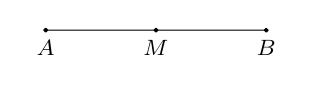
\begin{tikzpicture}[scale=0.7,line join=round,line cap=round,font=\footnotesize,>=stealth]
					\draw[fill = black] (0,0) circle (1pt)  node[below]{$A$}
						--  (2,0) circle (1pt) node[below]{$M$}
						-- (4,0) circle (1pt) node[below]{$B$}; 
				\end{tikzpicture}
		\end{center}
		Hai vectơ đối nhau  là hai vectơ cùng độ dài và ngược hướng nên nhìn vào hình vẽ ta thấy vectơ cùng độ dài và ngược hướng với vectơ $\overrightarrow{AM}$ là $\overrightarrow{BM}$.
	} 
\end{ex}
